\section{Teorema de Bayes}

\subsection{O que é o Teorema de Bayes?}

O teorema de Bayes fornece um modo de calcular a probabilidade de uma hipótese baseado na probabilidade de outras hipóteses \textbf{a priori}.

\subsection{Fórmula do Teorema de Bayes}

\[ \large P(A|B) = \frac{P(A) \cdot P(B|A)}{P(B)}\]

\begin{itemize}
\item $P(A|B)$: probabilidade do evento 'A' ocorrer dado que 'B' ocorreu
\item $P(A)$: probabilidade de 'A' ocorrer
\item $P(B|A)$: probabilidade do evento 'B' ocorrer dado que 'A' ocorreu
\item $P(B)$: probabilidade de 'B' ocorrer
\end{itemize}

Portanto, o Teorema de Bayes afirma que a probabilidade posterior do evento A (ou seja, a probabilidade do evento A dado que o evento B ocorreu) é igual à probabilidade contrária P(B \(|\) A) multiplicada pela probabilidade de A e dividido pela probabilidade de B.

\subsection{Teorema de Bayes utilizando Scikit-Learn no Python}

Vamos utilizar um conjunto de dados que incluem 4 observações sobre um determinado momento do dia (clima - claro, chuvoso ou geada; feriado ou dia útil; período - manhã, horário de almoço ou noite; houve ou não congestionamento) e, a partir desses dados base, tentaremos prever a probabilidade de acontecer um congestionamento utilizando valores fornecidos apenas das 3 condições iniciais. Para isso, usaremos a biblioteca \textbf{Scikit-Learn} do Python.

\begin{minted}{python}
def getTempo():
return ['Claro', 'Claro', 'Claro', 'Claro', 'Claro', 
'Claro', 'Chuvoso', 'Chuvoso', 'Chuvoso', 'Chuvoso', 
'Chuvoso', 'Chuvoso', 'Geada', 'Geada', 'Geada', 'Geada', 
'Geada', 'Geada']

def getDiaSem():
return ['Útil', 'Útil', 'Útil',
'Feriado', 'Feriado', 'Feriado',
'Útil', 'Útil', 'Útil',
'Feriado', 'Feriado', 'Feriado',
'Útil', 'Útil', 'Útil',
'Feriado', 'Feriado', 'Feriado']

def getHorario():
return ['Manhã', 'Almoço', 'Noite',
'Manhã', 'Almoço', 'Noite',
'Manhã', 'Almoço', 'Noite',
'Manhã', 'Almoço', 'Noite',
'Manhã', 'Almoço', 'Noite',
'Manhã', 'Almoço', 'Noite']

def getCongest():
return ['Sim', 'Não', 'Sim',
'Não', 'Não', 'Não',
'Sim', 'Sim', 'Sim',
'Não', 'Não', 'Não',
'Sim', 'Sim', 'Sim',
'Sim', 'Não', 'Sim']

Tempo = getTempo()
diaDaSem = getDiaSem()
Horario = getHorario()
Congest = getCongest()

pd.DataFrame(zip(Tempo,diaDaSem,Horario,Congest), 
columns=['Tempo','Dia da semana',
'Horário','Congestionamento'])
\end{minted}

\begin{table}[H]
	\centering
	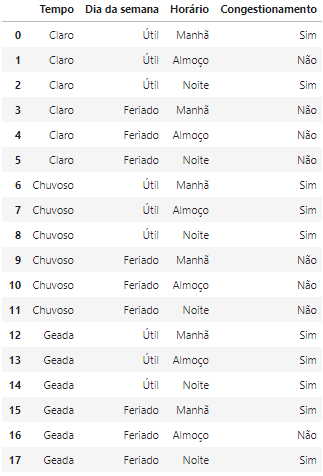
\includegraphics[width=0.6\textwidth]{./Imagens/Teorema de Bayes/Tabela.png} 
	\caption{Condições do dia}
	\label{tab:Condições do dia}
\end{table}

\subsubsection{Pré-processamento dos dados}

Vamos utilizar o comando 'sklearn.preprocessing.LabelEncoder' para \textbf{normalizar} os dados, ou seja, alterar os valores das colunas numéricas no conjunto de dados para uma escala comum, sem distorcer os intervalos de valores ou provocar perda de informações. No exemplo analisado, os valores do tipo texto serão transformados em valores numéricos. Ainda, usamos o método \textbf{fit\textunderscore transform()} para evitar possíveis erros que poderiam ser provocados por valores nulos, inexistentes ou indefinidos no nosso conjunto de dados. Por fim, organizamos os dados relevantes (\textbf{features}) para o nosso exemplo em uma única lista.

\begin{minted}{python}
labelEncoder = preprocessing.LabelEncoder()
# Normalizando e aplicando o 'fit_transform'
normTempo = labelEncoder.fit_transform(Tempo)
normDiaDaSem = labelEncoder.fit_transform(diaDaSem)
normHorario = labelEncoder.fit_transform(Horario)
normCongest = labelEncoder.fit_transform(Congest)
print("-----------------normalização-----------------")
print(normTempo)
print(normDiaDaSem)
print(normHorario)
print(normCongest)
# Organizando os dados relevantes (features)
features = []
for i in range(len(normTempo)):
	features.append([normTempo[i], normDiaDaSem[i], 
	normHorario[i]])
print("-----------------features-----------------")
print(features)
# Aplicando o Método de Bayes
modelo = GaussianNB()
# Treinando o modelo
modelo.fit(features, normCongest)
\end{minted}

\subsubsection{Fazendo as predições}

\begin{minted}{python}
# ["Geada", "Útil", "Manhã"]
print(modelo.predict([[2, 1, 1]]))
# resultado = [1]
# ["Claro", "Feriado", "Almoço"]
print (modelo.predict([[1, 0, 0]]))
# resultado = [0]
\end{minted}

Portanto, para as condiçoes ["Geada", "Útil", "Manhã"] por exemplo, há uma grande probabilidade de ocorrer congestionamento.
Para as condiçoes ["Claro", "Feriado", "Almoço"], a probabilidade de ocorrer um congestionamento é baixa.

\subsection{Aplicações do Teorema de Bayes}

\begin{itemize}
\item Aprendizado de máquinas, principalmente nas classificações de dados.
\item Pode ser utilizado na química para avaliar a densidade de probabilidade da composição química de um sistema em termos das densidades de probabilidade das abundâncias das diferentes espécies químicas.
\item Pode ser utilizado para prever a qualidade de água com base na concentração de toxinas e outros poluentes que possam ultrapassamr os limites numéricos do padrão de qualidade da água.
\item Em engenharia estrutural, auxiliando o engenheiro a determinar se a estrutura é segura ou não, com base nos valores de reabilidade. 
\end{itemize}



